\chapter{A Multi-view Framework for System Modeling\label{chapter:framework}}

This chapter introduces the necessary background on modeling formalisms and techniques used in this thesis. It is organized as follows. The running example used throughout the thesis is briefly presented in the next section. Section~\ref{section:background-multi-agent-systems-and-behavior-modeling} then provides a general overview of the modeling framework, its main hypotheses, and how multiple models fit together. The models and their semantics are then detailed in subsequent sections. Section~\ref{section:background-state-machines} introduces the state machines considered in this thesis. Scenarios and related constructs are defined in Section~\ref{section:background-scenarios}. To integrate event-based and state-based specifications, fluents are introduced in Section~\ref{section:background-fluents}. The fluent-based specification of goals and domain properties is discussed in Section~\ref{section:background-goals}. Section~\ref{section:background-process-models} introduces guarded process models. Section~\ref{section:background-discussion} concludes this chapter with an overview of model synthesis opportunities offered by the present framework.

\section{Running example: A toy train system\label{section:background-running-example}}

We use a simple train system fragment as running example for illustrating concepts and techniques throughout this thesis. The system is composed of an automated train controller, actuators for doors and the engine as well as the latter themselves, sensors, and a passenger. Via the actuators, the controller typically controls operations like starting or stopping the train, opening or closing the doors, and so on. A safety goal requires train doors to remain closed while the train is moving. If the train is not moving and the passenger presses the alarm button, the controller must open the doors immediately. If the train is moving and the passenger presses the alarm button, then the controller must stop the train first and then open the doors. Typical agent interactions for the latter case are depicted in Fig.~\ref{image:train-scenario-all-agents}. The precise semantics of such a scenario is made clear in the following sections.

\begin{figure}\centering
\scalebox{0.75}{
  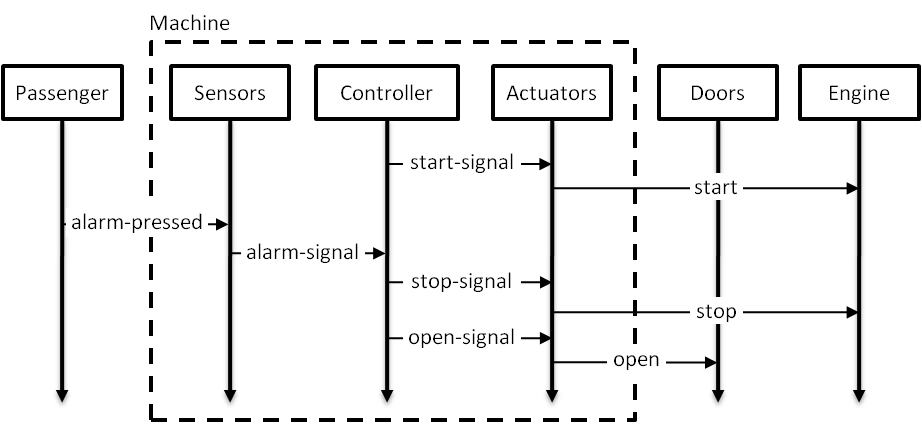
\includegraphics[trim=2mm 2mm 2mm 2mm, clip]{src/2-framework/images/train-scenario-all-agents}
}
\caption{A scenario illustrating a train system stopping in emergency when an alarm is pressed.\label{image:train-scenario-all-agents}}
\end{figure}


\section{Framework overview\label{section:background-multi-agent-systems-and-behavior-modeling}}

Modeling software systems calls for rich models that cover the structural, intentional and behavioral dimensions of the system~\cite{VanLamsweerde:2000}. Our framework integrates these co-related dimensions with an emphasis on the behavioral one. We start with a guided tour along those dimensions before discussing how multiple models actually fit together in a coherent way.

\subsection{Capturing multiple views of the system\label{subsection:background-multiple-views}}

%%% The structural view

\noindent \textbf{The structural view} -- A system is commonly seen as being made of active components, called \emph{agents}, that behave and interact so as to fulfill system goals; they need to restrict their behavior so as to ensure the goals they are responsible for~\cite{Feather:1987}. Some of them are human agents (e.g. passenger in Fig.\ref{image:train-scenario-all-agents}); others are physical or electronic devices (e.g. train doors and actuators); others are software components (the software controller).

In addition to the notion of \emph{system}, that encompasses all agents, the literature makes use of specific terms to distinguish between certain agents and/or agent aggregations. In~\cite{VanLamsweerde:2009} for example, the \emph{software-to-be} denotes software agent(s) that need to be developed (the automated controller, for example) while the other agents compose its \emph{environment}. Another boundary consists in distinguishing the software together with its input and output devices from the other agents. This boundary, depicted with a dashed line in Fig.~\ref{image:train-scenario-all-agents}, corresponds to the distinction made by Jackson between the \emph{world} and the \emph{machine}~\cite{Jackson:1995}.

This thesis sticks to very basic notions of structural modeling. The interfaces among the agents composing the system consist of messages, called \emph{events}, that the agents can send or receive (see the behavioral dimension below). By simplicity we assume that event labels uniquely determine agent interactions. We do not consider specific abstractions for modeling agent interfaces and boundaries, like context diagrams~\cite{Jackson:1995} and events structured in terms of attributes.

A set of agents can be aggregated into a new one of coarser granularity. Therefore, events can be partitioned among internal, boundary and external events. The boundary events form the new agent's interface. The surrounding box can be seen as a white or a black-box, dependent on whether internal events are shown or hidden, respectively. The composition and hiding operators on state machines, introduced below, support such structural mechanisms on the behavioral side. For a more precise description of structural models that nicely fit this framework the reader can refer to~\cite{Magee:1995}.

%%% The behavioral view

\noindent \textbf{The behavioral view} -- Behaviors capture the dynamic interactions among the agents forming the system; they will be modeled as sequences of events. In an interaction, an event is \emph{synchronously} sent by a source agent and received by a target agent. The same event can in fact be received by several agents at once; a form of \emph{broadcasting} is thus supported. 

Typical examples and counterexamples of system behaviors are specified through positive and negative scenarios involving agent instances, like the one in Fig.~\ref{image:train-scenario-all-agents}. The Message Sequence Charts (MSC) notation will be used to capture scenarios~\cite{ITU:1996}. Higher-level scenarios will be supported by introducing sequences and loops in such descriptions.

In addition to the partial behavior description linking agent instances, the complete behavior of each agent will be modeled at class level through a form of state machine known as labeled transition systems (LTS)~\cite{Keller:1976, Milner:1989}. The behavior of the entire system is obtained by parallel composition~\cite{Hoare:1985} of the agent LTSs. Behavior  projection on specific agents is also supported, in order to get the zoom-in/zoom-out facilities as suggested before.

This thesis will focus on \emph{determinate} agents~\cite{Engelfriet:1985}; these are agents whose observable behavior can be captured with the sole use of \emph{deterministic} transition systems (see Section~\ref{section:background-state-machines}).
\begin{itemize} 
\item This restriction results in a simple and intuitive framework, for easier accessibility to stakeholders involved in the early phases of system design. 
\item It also allows us to formalize behaviors with standard \emph{trace theory} \cite{Hoare:1985} and stick ourselves to the simplest notion of behavior equivalence, namely \emph{trace equivalence}~\cite{Engelfriet:1985}. 
\item Agent and system behaviors can then be captured by the class of \emph{prefix-closed} regular languages, a subclass of the well-studied \emph{regular} languages~\cite{Hopcroft:1979, Aho:1986}. Further to enabling the reuse of standard results from automaton theory, this paves the way to using grammar inference~\cite{Gold:1978} for behavior model synthesis (see chapter~\ref{chapter:inductive-synthesis}). 
\end{itemize}

%%% The intentional view

\noindent \textbf{The intentional view} -- This view is aimed at capturing \emph{why} the system is needed. A \emph{goal} is a prescriptive statement of intent whose satisfaction requires the collaboration of system agents. Unlike goals, \emph{domain properties} are descriptive statement about the environment -- such as physical laws, organizational rules, etc. Goal models are AND/OR graphs that capture how functional and non-functional goals contribute positively or negatively to each other~\cite{VanLamsweerde:2000, VanLamsweerde:2004}.

The thesis will focus on behavioral goals. A \emph{behavioral} goal implicitly defines a maximal set of admissible system behaviors. Unlike \emph{soft} goals, such goals can be established in a clear-sense (refer to~\cite{VanLamsweerde:2009} for a taxonomy of goals). For model synthesis the thesis will only consider goals and domain properties that can be formalized as \emph{safety} properties in linear temporal logic (LTL)~\cite{Manna:1992}. A safety property stipulates that some ``bad thing'' may not happen. If such a ``bad thing'' happens in an infinite sequence, then it must also do so after some finite prefix and must be irremediable~\cite{Alpern:1986, Giannakopoulou:1999}. Interestingly, the class of system behaviors satisfying safety properties can be expressed through labeled transition systems; behavioral goals and domain properties can therefore be integrated in our framework without much additional machinery.

For the modeller, goals are best captured through state-based abstractions (e.g. ``the train may be \emph{moving} only if the doors are \emph{closed}''). In contrast, the formal behavioral view is event-based (e.g. ``the train controller starts and stops the engine''). \emph{Fluents} will be used as an effective way for reconciling these two paradigms~\cite{Miller:2002}; they capture state-based propositions in terms of the occurrence of events. Behavioral goals will therefore be formalized in Fluent Linear Temporal Logic (FLTL)~\cite{Giannakopoulou:2003}, a flavor of linear temporal logic where atomic propositions are fluents. The structuring of goals in goal graphs and their assignment to agents will not be considered in the thesis.

%%% The operational view

\noindent \textbf{The operational view} -- This view aims at capturing processes which agents are involved in. Processes are made of tasks and decisions. A task is a unit of work to be performed by the collaboration of the agents. A decision is a condition on the process state which drives which tasks are to be performed next.

The guarded high-level Message Sequence Charts (g-hMSC) notation will be used to capture processes~\cite{Damas:2009, Damas:2011}. Tasks in a g-hMSC are either MSC scenarios or finer-grained g-hMSCs. Decision nodes capture conditions on the process state in terms of fluents. The semantics of g-hMSC will be defined in Chapter~\ref{chapter:deductive}.

%%% Double, double, double

\subsection{On the double use of labeled transition systems}

The multi-view framework depicted in Fig.~\ref{image:framework} provides a key for reading the rest of this chapter. As we put more emphasis on behavior modeling, all models will be grounded on standard trace theory~\cite{Hoare:1985}. \emph{Traces} are finite sequences of event labels. They will be used to capture the system behaviors described in a MSC scenario, those admitted by a behavioral goal, and so on. Labeled transition systems (LTS) will allow us to capture and manipulate \emph{sets} of traces. A trace-based semantics will provide precise answers to questions such as:

\begin{itemize} 
\item what agent and system traces does this scenario cover?
\item is this trace accepted by this state machine?
\item does this sequence of events violate this behavioral goal?
\end{itemize}

Note that labeled transition systems appear twice on the figure, as we will make two different uses of them. 

\begin{itemize} 
\item LTS provide a representation for the sets of traces that capture model semantics. 
\item They are chosen as a particular representation for agent state machines (even though one could argue that such a representation is too low-level to be accessible to stakeholders).
\end{itemize}

As a consequence, we may consider the model synthesis problem from two different perspectives:

\begin{itemize}
\item to generate low-level models for defining the semantics of higher-level ones, as to analyze the latter~\cite{Magee:1997, Uchitel:2003, Damas:2009};
\item to generate missing views in a multiview modeling framework, or to complete them~\cite{VanLamsweerde:1998, Whittle:2000, Uchitel:2004, Damas:2005}.
\end{itemize}

\begin{figure}[t]\centering
  \scalebox{0.50}{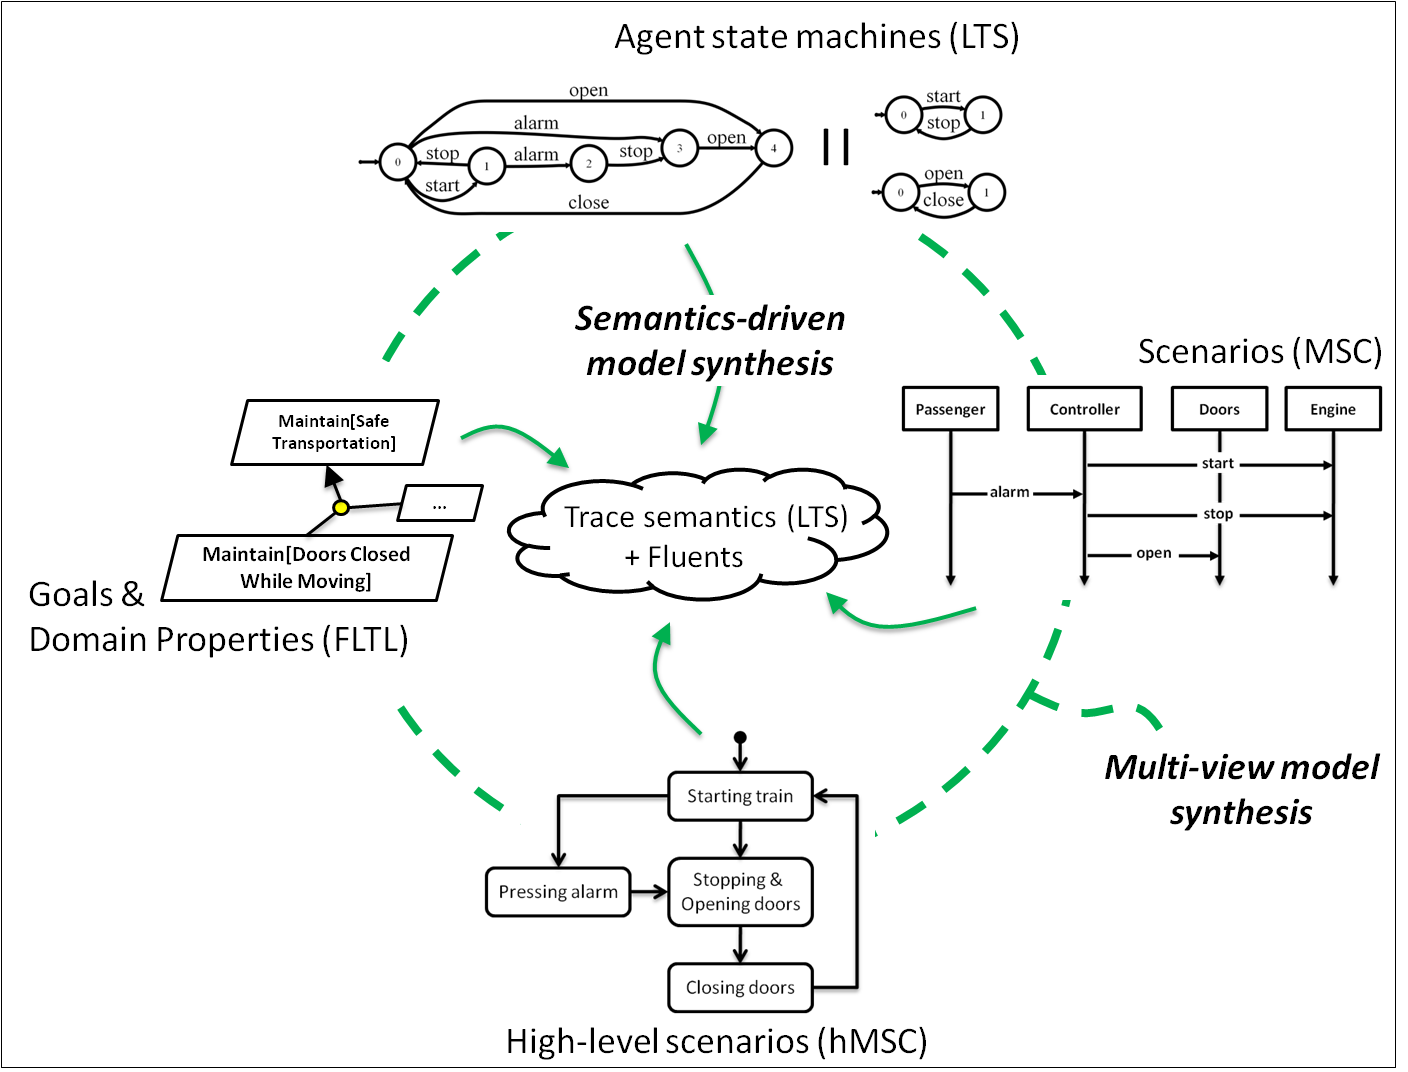
\includegraphics[trim=2mm 2mm 3mm 2mm, clip]{src/2-framework/images/framework}}
  \caption{Formal framework outline.\label{image:framework}}
\end{figure}



\section{State machines as labeled transition systems\label{section:background-state-machines}}

In our framework, the behavior of an agent will be modeled by a specific kind of finite state machine called \emph{labeled transition system} (LTS). This formalism, initially introduced by Keller for reasoning about parallel programs~\cite{Keller:1976}, has been intensively used for specifying and analyzing concurrent systems, e.g. in~\cite{Milner:1989, Clarke:1989, Magee:1997}. 

A LTS is made of a set of states and a set of transitions between them (see Fig.~\ref{image:framework-start-stop}). Each transition has an \emph{event} label -- sometimes called \emph{symbol} or \emph{action} label. A state is labeled with a number to distinguish if from other states. An \emph{initial state} is designated graphically by an incoming arrow with no source state (e.g. state 0 in Fig. \ref{image:framework-start-stop}). 

\begin{figure}[H]
\centering\scalebox{0.60}{
  \includegraphics*[clip]{src/2-framework/images/start-stop}}
  \caption{A Labeled Transition System for an \artifact{Engine} agent\label{image:framework-start-stop}.}
\end{figure}

\begin{definition}[Labeled Transition System]
A LTS is defined as a 4-tuple $(Q,\Sigma,\delta,q_{init})$ where
\begin{itemize}
\item $Q$ is a finite set of states,
\item $\Sigma$ is a set of labels called its \emph{alphabet}, 
\item $\delta$ is a transition relation $Q \times \Sigma\cup\{\tau\} \times Q$,
\item $q_{init} \in Q$ is the initial state. 
\end{itemize}
\end{definition}

The \emph{alphabet} $\Sigma$ captures the notion of \emph{agent interface} as a set of event labels that an agent recognizes. These are the events in which the agent \emph{engages} in synchronous communications with its environment. For example, the LTS in Fig.~\ref{image:framework-start-stop} has an alphabet \artifact{$\Sigma=\{start, stop\}$}. 

The set of finite sequences over an alphabet $\Sigma$ will be denoted by $\Sigma^{*}$.

The label $\tau$ in the above definition of a LTS is used to denote so-called \emph{non-observable} transitions. Such transitions allow us to model agent state changes that cannot be monitored by its environment. We will denote $\Sigma\cup\{\tau\}$ by $\Sigma_{\tau}$, refering then to an alphabet augmented with the $\tau$ label.

Note that LTS do not distinguish between \emph{sent} and \emph{received} events. Such distinction may be required when connecting them with scenarios. In such cases, we assume this structural information to be available elsewhere, typically, from a context or architecture diagram~\cite{Ward:1985, Magee:1995}. We will also assume that an event label uniquely determines the interacting agents; an event may however be received by more than one of them. 

\begin{definition}[Trace]
Given an alphabet $\Sigma$, a \emph{trace} is an element of $\Sigma^{*}$, that is, a finite sequence of event labels \artifact{$w = \textless l_0,\ldots,l_{n} \textgreater$} with $l_i \in \Sigma$. We will sometimes use the notation $vw$ to denote the concatenation of a trace $v$ with another trace $w$.
\end{definition}

\begin{definition}[Deterministic LTS]
A LTS is \emph{deterministic} if a trace always uniquely determines the reached state; otherwise it is \emph{non-deterministic}. A deterministic LTS may therefore not have $\tau$ transitions; neither does it have a state with two outgoing transitions sharing the same label, that is, 
\begin{center}$(q,l,q_1) \in \delta \wedge (q,l,q_2) \in \delta \implies q_1 = q_2$\end{center}
\end{definition}

\begin{definition}[Terminating LTS]
A state is \emph{terminating} if it has no outgoing transition; otherwise it is \emph{non-terminating}. A \emph{terminating} LTS has at least one terminating state; otherwise it is \emph{non-terminating}. 
\end{definition}

Note that the above definition does not allow distinguishing between terminating states that capture successful termination (where an agent stops running intentionally) and non-successful termination (e.g., an agent composed from finer-grained agents \emph{deadlocks} unintentionally). Deadlock analysis will be left outside the scope of the thesis.

\begin{definition}[LTS execution]
A \emph{LTS execution} is a finite sequence of states separated by labels:
\begin{center}
\artifact{$w = \textless q_0,l_0,\ldots,q_{n-1},l_{n-1},q_n \textgreater$} 
\end{center}
\noindent with $q_i \in Q$ and $l_i \in \Sigma_{\tau}$. 
\end{definition}

The \emph{projection} of an execution $w$ over an alphabet $\Sigma$, denoted by $w|_{\Sigma}$, is the result of keeping from $w$ only those event labels that belong to $\Sigma$ -- in other words, $q_i$ states and $\tau$ labels have been eliminated. The projection of an execution thus yields a trace. 

\begin{definition}[Valid LTS execution]
An execution is \emph{valid} for a LTS if it denotes a path from the initial state in the corresponding graph:
\begin{center}
$q_0 = q_{init}$ and $(q_i,l_i,q_{i+1}) \in \delta$ for $0 \leq i < n$. 
\end{center}
\end{definition}

\begin{definition}[Accepted trace]
A trace $t$ is \emph{accepted} by a LTS if there exists a valid execution $w$ such that $w|_{\Sigma} = t$. 
\end{definition}

In other words, a trace is accepted by a LTS if it denotes an existing path in the corresponding graph from the initial state, possibly with silent moves offered by $\tau$ transitions in the non-deterministic case -- in this case, a trace may actually denote more that one existing path. 

As a consequence of this definition, a prefix of an accepted trace is an accepted trace as well; the empty trace $\lambda$ is therefore always accepted. 

For example, the LTS in Fig.~\ref{image:framework-start-stop} accepts the trace \artifact{<start stop start>}, the trace \artifact{<start stop>}, but not the trace \artifact{<start start>}. 

\begin{definition}[Language of a LTS]
The set of traces accepted by a LTS $P$ is called its \emph{language}; it is denoted by $\mathcal{L}(P)$.
\end{definition}

For example, the language of the LTS shown in Fig.~\ref{image:framework-start-stop} is
\begin{center}
$\mathcal{L}(\artifact{Engine})=\{\lambda$, \artifact{<start>}, \artifact{<start stop>}, \artifact{<start stop start>}, \ldots $\}$
\end{center} 

\emph{Behavioral equivalence} is an important notion when designing and analyzing concurrent systems. It allows answering questions such as ``\emph{are agents $Ag_1$ and $Ag_2$ the same in terms of behavior?}''. Many different notions of behavioral equivalence exist in the literature, like \emph{strong} and \emph{observational}  equivalences~\cite{Milner:1989}, bisimilarity~\cite{Park:1981}, or failure equivalence~\cite{Hoare:1985}. Our assumption about \emph{determinate} agents, introduced in in Section~\ref{subsection:background-multiple-views}, allows us to stick to the weakest and simplest notion of LTS equivalence: trace equivalence~\cite{Hoare:1985, Engelfriet:1985}. 

\begin{definition}[Trace equivalence]
Two LTS $P$ and $Q$ are \emph{trace-equivalent} if they accept the same set of traces:
\begin{equation*}
P \equiv_{tr} Q \mbox{~if and only if~} \mathcal{L}(P) = \mathcal{L}(Q)
\end{equation*}
\end{definition}

The next section discusses some important properties inherited by LTSs from their connection with regular languages. 

\subsection{Labeled transition systems and regular languages\label{section:background-lts-and-regular-languages}}

Labeled transition systems are actually a subclass of finite automata \cite{Hopcroft:1979}. 

\begin{definition}[Finite automaton]
A finite automaton is a 5-tuple \\ $(Q,\Sigma,\delta,q_{init},F)$ where 
\begin{itemize}
\item $Q$ is a finite set of states, 
\item $\Sigma$ is an alphabet, 
\item $\delta$ is a transition relation $Q \times \Sigma\cup\{\tau\} \times Q$, 
\item $q_{init}$ is the initial state, and 
\item $F$ is a subset of $Q$ identifying the accepting states. 
\end{itemize}
\end{definition}

The only difference between LTS and finite automata is that the latter distinguish between \emph{accepting} and \emph{non-accepting} states, through $F \subseteq Q$. Accepting states are depicted with double circles. Only traces that end in an accepting state are accepted by a finite automaton.

A finite automaton is shown in Fig.~\ref{image:finite-automaton}. State 0 is accepting whereas state 1 is non-accepting. As a consequence, this automaton accepts the trace $\artifact{<a b b>}$ but not the trace \artifact{<a b>}.

\begin{figure}[H]
\centering\scalebox{0.50}{
  \includegraphics*[clip]{src/2-framework/images/finite-automaton}}
  \caption{A finite automaton\label{image:finite-automaton}.}
\end{figure}

A LTS is a standard automaton in which all states are accepting, that is $F = Q$. Many results from standard automata theory therefore apply to LTS while preserving trace equivalence.

Standard automata, deterministic or non-deterministic, capture the well-studied class of \emph{regular} languages~\cite{Hopcroft:1979}. As they only have accepting states, LTS capture the class of \emph{prefix-closed} regular languages. The term ``prefix-closed'' means that all prefixes of accepted traces are also accepted traces: 
\begin{equation*}
prefixes(\mathcal{L}(P)) = \mathcal{L(P)}
\end{equation*}

For any regular language $\mathcal{L}$, there exists a canonical automaton $A(\mathcal{L})$. This automaton is the minimal deterministic automaton accepting $\mathcal{L}$; it is known to be unique up to state renumbering~\cite{Hopcroft:1979}. 

Without loss of generality, we may therefore assume that the behavior of any agent is modeled by a canonical LTS. Moreover, we may use non-deterministic constructions, $\tau$ transitions in particular, without contradicting the assumption of \emph{determinate} agents. 

Given a LTS $P$, deterministic or not, we will denote by $P^{\Delta}$ its canonical equivalent, where $P$ can actually be a LTS \emph{expression}, that is, a LTS ``computed'' by applying LTS operators introduced in the next sections. Standard automaton algorithms from~\cite{Hopcroft:1979} can be used to compute $P^\Delta$. This typically involves removing $\tau$ transitions, determinizing and minimizing the LTS under trace equivalence.

As languages are sets of traces, it is sometimes natural to reason in terms of standard operators on sets. In the following sections, we will often make use of notations for the union of two languages ($\cup$), their intersection ($\cap$), subset ($\subseteq$), proper subset ($\subset$) and equality ($=$). Techniques and algorithms for implementing these operators for the general case of standard automata can be found in~\cite{Hopcroft:1979, Aho:1986}. 

For a given language $\mathcal{L}$, $mt(\mathcal{L})$ denotes the set of \emph{maximal} traces of $\mathcal{L}$, that is, traces that cannot be extended by a suffix within the same language. In the case of a deterministic LTS, they simply correspond to traces reaching a terminating state.

The next two sections define two additional operators, \emph{composition} and \emph{hiding}, that support reasoning about behaviors in presence of multiple agents with different alphabets.

\subsection{Systems as agent compositions\label{subsection:lts-composition}}

A system is composed of active agents whose behavior is explicitly modeled by a LTS. The behavior of the system itself is defined through parallel composition~\cite{Hoare:1985}. In this setting agents execute asynchronously but synchronize on shared events. A system made of $n$ agents is defined as:
\begin{equation}
System = Ag_1 \parallel \ldots \parallel Ag_n
\label{equation:parallel-composition}
\end{equation}

As we are mostly interested in agent \emph{behaviors}, for parallel composition we will use the binary composition operator $\parallel$ defined on LTS \cite{Giannakopoulou:1999, Magee:1999}. This operator computes the interleaving of all traces accepted by the two LTS under the constraint that they synchronize on shared labels. It is both commutative and associative, allowing us to write~(\ref{equation:parallel-composition}) without ambiguity. 

\begin{definition}[LTS composition]
Let $P = (S_1,\Sigma_1,\delta_1,q_{1})$ and $Q = (S_2,\Sigma_2,\delta_2,q_{2})$ denote two LTS. Their \emph{composition} is another LTS 
\begin{center}
$P \parallel Q = (S_1 \times S_2,\Sigma_1\cup\Sigma_2,\delta,(q_1,q_2))$
\end{center}
\noindent where $\delta$ is the smallest relation satisfying the following rules~\cite{Giannakopoulou:1999}:

\begin{center}
\begin{tabular}{cc}
$\frac{\displaystyle P \stackrel{l}{\longrightarrow} P'}{\displaystyle P \parallel Q \stackrel{l}{\longrightarrow} P' \parallel Q}~~l \notin \Sigma_2$ &
$\frac{\displaystyle Q \stackrel{l}{\longrightarrow} Q'}{\displaystyle P \parallel Q \stackrel{l}{\longrightarrow} P \parallel Q'}~~l \notin \Sigma_1$ \\
 & \\
\multicolumn{2}{c}{$\frac{\displaystyle P \stackrel{l}{\longrightarrow} P',~Q \stackrel{l}{\longrightarrow} Q'}{\displaystyle P \parallel Q \stackrel{l}{\longrightarrow} P' \parallel Q'}~~l \neq \tau$} \\
\end{tabular}
\end{center}
The notation $X \stackrel{l}{\longrightarrow} X'$ means that the LTS $X = (S,\Sigma,\delta,q_0)$ may \emph{transit} into another LTS $X' = (S,\Sigma,\delta,q_1)$ through the event label $l$, provided that $(q_0,l,q_1) \in \delta$. 
\end{definition}

$P \parallel Q$ is thus defined on the Cartesian product of the sets of states of $P$ and $Q$; its initial state is $\{q_1,q_2\}$. The above rules define the possible transitions from such a state. 

\begin{itemize}
\item The first two rules are symmetric; they encode the fact that, on non-shared labels, one LTS may transit while the other stays in its previous state. Those rules allow individual LTS to move along their $\tau$ transitions. 
\item The last rule forces the two LTS to transit together on all shared labels but $\tau$.
\end{itemize}

A composed LTS can be easily computed constructively by exploring the state space from its initial state until no new state pair is discovered. 

When the two LTS operands share the same alphabet, the composition operator computes the intersection of accepted traces:
\begin{equation*}
\mathcal{L}(P \parallel Q) = \mathcal{L}(P) \cap \mathcal{L}(Q) \mbox{~~if~~} \Sigma_{1}=\Sigma_{2}
\end{equation*}

The trace semantics of a system composed of $n$ agents whose behavior is modeled with LTSs $Ag_1 \ldots Ag_n$ is captured by:
\begin{equation}
\mathcal{L}(System) = \mathcal{L}(Ag_1 \parallel \ldots \parallel Ag_n)
\label{equation:system-composition}
\end{equation}

\subsection{Black-box behavior through event \emph{hiding}\label{subsection:lts-hiding}}

It is sometimes useful to consider the composition of a subset of agents that together define an interesting boundary in the system considered. 

Consider the agents depicted in the scenario of Fig.~\ref{image:train-scenario-all-agents}, for example. The machine boundary can simply be modeled as follows:
\begin{align*}
Machine &= Controller \parallel Actuators \parallel Sensors \\
World   &= Passenger \parallel Doors \parallel Engine \\
System  &= Machine \parallel World
\end{align*}

As seen before, the $Machine$ agent has an interface in terms of the set of events in which it engages. This interface might be too large. A black-box version of the $Machine$ behavior might be suitable; it is a LTS whose interface is restricted to those events crossing the depicted boundary.

\begin{definition}[LTS hiding]
The \emph{hiding} of a set of labels $I$ in a LTS $P = (Q,\Sigma,\delta,q_{init})$ defines the LTS:
\begin{center}
$P \setminus I = (Q,\Sigma \setminus I,\delta_{hidden},q_{init})$
\end{center}
\noindent where $\delta_{hidden}$ is the smallest relation satisfying the following rules~\cite{Giannakopoulou:1999}:
\end{definition}

\begin{center}
\begin{tabular}{cc}
$\frac{\displaystyle P \stackrel{l}{\longrightarrow} P'}{\displaystyle P \setminus I \stackrel{l}{\longrightarrow} P' \setminus I}~~l \notin I$ & 
$\frac{\displaystyle P \stackrel{l}{\longrightarrow} P'}{\displaystyle P \setminus I \stackrel{\tau}{\longrightarrow} P' \setminus I}~~l \in I$ \\
\end{tabular}
\end{center}

The hiding operator thus makes a set of labels invisible to the environment by replacing them by $\tau$ transitions. The resulting LTS is non-deterministic. However, a minimal and deterministic equivalent exists as discussed in the previous section. 

In our example, the LTS of the black-box machine we are actually looking for is:
\begin{align*}
\mbox{\emph{Machine'}} &= (\mbox{\emph{Machine}} \setminus \mbox{\emph{Internals}})^\Delta~,
\end{align*}

\noindent where \emph{Machine} is the composition between the controller, actuators and sensors given previously and \emph{Internals} is the set of events internal to the machine -- here, $\{\artifact{start-signal}, \artifact{stop-signal}, \artifact{open-signal}, \artifact{alarm-signal}, \ldots\}$ (see Fig.~\ref{image:train-scenario-all-agents}).

Given a LTS $P = (Q,\Sigma,\delta,q_{init})$ and a set of labels $I$, the relation between the languages of $P$ and $P \setminus I$ is defined as follows:
\begin{equation*}
\mathcal{L}(P \setminus I) = \{ t'~|~\exists t \in \mathcal{L}(P)~such~that~t' = t|_{\Sigma \setminus I}\}
\end{equation*}

That is, the traces accepted by $P \setminus I$ are the projections of those accepted by $P$ on the restricted alphabet $\Sigma \setminus I$.

\section{Scenarios as message sequence charts\label{section:background-scenarios}}

Labeled transition systems may capture the behaviors of a single agent class. Scenarios illustrate admissible interactions among multiple agent instances. The scenarios we use in this thesis are specified in a syntactic subset of Message Sequence Charts (MSC)~\cite{ITU:1996}, see Fig.~\ref{image:train-scenario-all-agents} for an example. 

To keep scenario specifications accessible to end-users, we will consider only a small subset of their features. In its simplest form, a MSC is composed of vertical lines representing timelines associated with agent instances and horizontal arrows representing interactions events among them. According to the previous section, events are synchronously sent and received by interacting agents (we will also use the terms \emph{controlled} and \emph{monitored} events, respectively). We assume that an event label uniquely determines the latter agents. 

We consider \emph{positive} scenarios, that are examples of behaviors that the system should exhibit (see Section~\ref{subsection:background-positive-scenarios}), and \emph{negative} scenarios that are counterexample behaviors that the system must avoid (see Section~\ref{subsection:background-negative-scenarios}). Sections~\ref{subsection:background-scenario-collections} and \ref{subsection:background-hmsc} will discuss ways of managing multiple positive and negative scenarios. The consistency of the scenarios and state machines views is discussed in Section~\ref{subsection:background-scenario-consistency}.

\subsection{Positive scenarios\label{subsection:background-positive-scenarios}}

As in~\cite{Uchitel:2004}, MSCs are given a trace semantics. We will consider that a MSC defines a set of traces; the latter are expressed through a LTS. Two kinds of traces are considered: those from the local perspective of a single timeline and those from the global perspective of the complete MSC. We discuss each of these views in turn.

As time in a MSC evolves from top to bottom, the order in which events are sent and received along a particular timeline defines a total order. Therefore, from the perspective of a single agent, a MSC defines one simple trace; such trace is a \emph{maximal} trace in that it includes all events in which the agent participates. This trace and all its suffixes can be captured by a LTS. Given a MSC $M$ and an agent $Ag$, we will denote such LTS by $M_{\downarrow Ag}$.

For example, the traces defined by the timeline of the \artifact{Controller} in the MSC of Fig.~\ref{image:train-scenario-all-agents} are precisely captured by the LTS in Fig.~\ref{image:local-traces-lts}. 

\begin{figure}\centering
\scalebox{0.45}{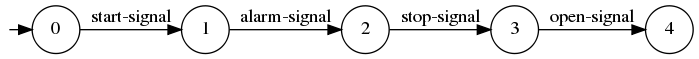
\includegraphics{src/2-framework/images/local-trace}}
\caption{LTS capturing the traces of the MSC in Fig.~\ref{image:train-scenario-all-agents} from the local perspective of the \artifact{Controller} agent.\label{image:local-traces-lts}}
\end{figure}

When looking at traces from the perspective of the whole MSC, two possibilities might be envisaged.

\noindent \textbf{Total event ordering} -- One might consider that a MSC defines a simple \emph{maximal} trace where all events appear according to the graphical top-down ordering. In the example of Fig.~\ref{image:train-scenario-all-agents}, such trace would be

\begin{center}\artifact{<start-signal, start, alarm-pressed, \ldots, open>}\end{center} 

A MSC would then define a total order among all events. This leads to a straightforward but limited trace semantics for MSCs.

\noindent \textbf{Partial event ordering} -- When considering concurrent systems, a partial ordering among events appears more adequate~\cite{ITU:1996, Uchitel:2003}. 

Consider for example the events \artifact{start-signal} and \artifact{alarm-pressed} at the beginning of the MSC shown in Fig.~\ref{image:train-scenario-all-agents}. These two events capture unrelated message passing between different agents; therefore, they can not be considered strictly ordered over time -- e.g. the passenger might push the alarm button when the \artifact{start-signal} is already sent but before \artifact{start} has been propagated; or maybe even before \artifact{start-signal}; and so on. 

To account for such situations, one has to consider that the traces defined by a MSC are \emph{linearizations} of the partial order among MSC events \cite{Alur:2000}. In other words, linearizations capture all possible sequences of events that respect the total ordering defined by the timelines. We do not formalize the structure of Message Sequence Charts and their linearizations here, and refer to~\cite{Uchitel:2003} for such mathematical characterization. 

Let $M$ denote a MSC. The set of traces it defines from the local and global perspectives are related as follows:
\begin{align}
\mathcal{L}_{total}(M) & \subseteq \mathcal{L}_{partial}(M) 
\label{equation:msc-composition-1} \\
\mathcal{L}_{partial}(M) &= \mathcal{L}(M_{\downarrow Ag_1} \parallel \ldots \parallel M_{\downarrow Ag_n})
\label{equation:msc-composition}
\end{align}

\begin{itemize}
\item Relation (\ref{equation:msc-composition-1}) states that the set of traces under a partial ordering includes those under a total ordering. Clearly, the model with partial ordering is more general than the one with total ordering. This means that everything that is true for the former is also true for the latter. Unless stated otherwise, we will therefore assume the general framework with partial ordering. In particular, we will no longer make the $partial$ and $total$ subscripting explicit when stating other language relations in the following sections.

\item Relation (\ref{equation:msc-composition}) provides a way of computing all linearizations of a MSC as an acyclic transition system through LTS composition. Such LTS is illustrated in Fig.~\ref{image:msc-linearizations} for the MSC in Fig.\ref{image:train-scenario-all-agents}. As shown there, the latter accepts six different linearizations due to the possible interleavings of its first four events. By construction, such LTS has only one initial state (the leftmost one) and only one terminating state (the rightmost one).
\end{itemize}

Note that the number of linearizations of a MSC is exponential in the number of events in the worst case. This is representative of distributed systems where agents generally behave asynchronously. Linearizations capture all possible interleavings of events in exactly the same way as LTS composition in Section~\ref{subsection:lts-composition}. In the worst case where agents do not synchronize at all, the number of interleavings is exponential. In practice, as they specifically illustrate agent interactions, MSCs often have only a few linearizations.

\begin{figure}\centering
\scalebox{0.29}{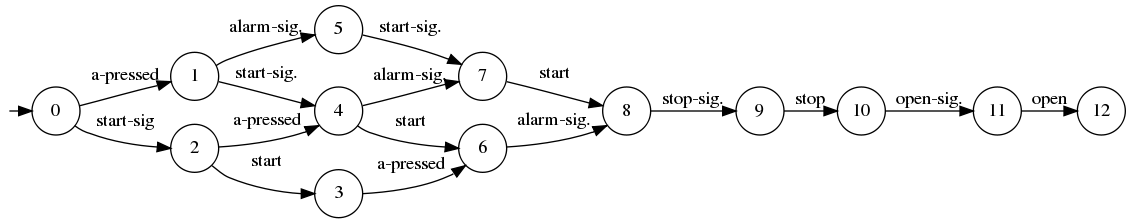
\includegraphics{src/2-framework/images/linearizations}}
\caption{LTS capturing all event linearizations of the MSC in Fig.~\ref{image:train-scenario-all-agents}. Here, \artifact{alarm-pressed} is abbreviated as \artifact{a-pressed} and \artifact{sig.} stands for \artifact{signal}. \label{image:msc-linearizations}}
\end{figure}

\subsection{Negative scenarios\label{subsection:background-negative-scenarios}}

Positive MSCs capture examples of behavior that the system is expected to exhibit. In addition, it is often convenient to specify examples of behavior that the system may \emph{not} exhibit. Proscribed behaviors are illustrated through negative MSCs~\cite{Uchitel:2002, Uchitel:2004}. A negative MSC is a scenario whose last event is prohibited, as depicted by a crossed arrow below a dashed line. Fig.~\ref{image:train-negative-scenario} shows a negative scenario where the \artifact{Controller} may not open doors immediately after having started the train.

\begin{figure}
\centering
\scalebox{0.75}{
  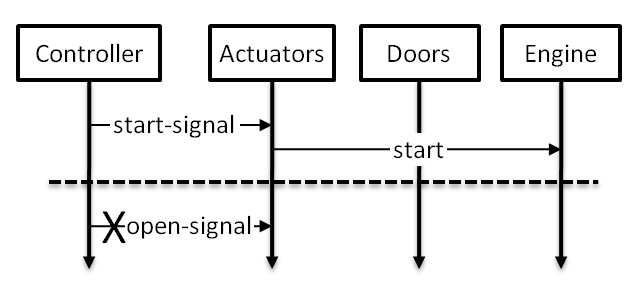
\includegraphics[trim=2mm 2mm 2mm 2mm, clip]{src/2-framework/images/train-negative-scenario}
}
\caption{A negative scenario illustrating that the controller may not open doors after having started.\label{image:train-negative-scenario}}
\end{figure}

More precisely, a negative MSC is a pair $(P,e)$ where $P$ is a positive MSC and $e$ is a single event label. The positive scenario prefix $P$ is called the $precondition$ and $e$ the \emph{prohibited event}. The intuitive semantics is that, once the precondition has occurred from the system's initial state, $e$ may not be the very \emph{next} event in the system. 

We now make the trace semantics of negative MSCs precise. First, the precondition of a negative MSC $N = (P,e)$ is a positive MSC; it therefore defines a set of positive traces $\mathcal{L}^{+}$:
\begin{align}
\mathcal{L}^{+}(N) = \mathcal{L}(P)
\end{align}

As in previous section, we consider the general framework with partial ordering here.

A negative MSC $N = (P,e)$ defines a set of negative traces $\mathcal{L}^{-}$:
\begin{align}
\mathcal{L}^{-}(N) &= \{~we \mid w \in mt(\mathcal{L}(P))~\}
\end{align}
\noindent where $mt(\mathcal{L})$ was seen to denote the set of maximal traces of the language $\mathcal{L}$ (see Section~\ref{section:background-lts-and-regular-languages}).

Negative traces are thus maximal traces of the precondition concatenated with the label of the proscribed event. Note that the precondition must occur completely for the prohibited event to be taken into account. In other words, partial orderings between the prohibited event and those in the precondition are not considered. This is the intended meaning of the dashed line separating them~\cite{Uchitel:2004}. 

Note that the negative language of a negative MSC cannot be captured through a pure LTS. This is because $\mathcal{L}^{-}(N)$ is not prefix-closed (see Section~\ref{section:background-lts-and-regular-languages}). Negative scenarios are sometimes captured by a LTS extended with an error state, see Fig.~\ref{image:negative-trace-lts} where the error state is depicted in black. Alternatively, we may use a standard automaton that makes a distinction between accepting and non-accepting states.

\begin{figure}\centering
\scalebox{0.45}{
  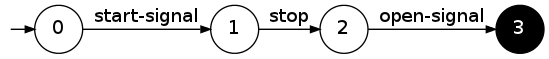
\includegraphics[trim=1mm 1mm 1mm 1mm, clip]{src/2-framework/images/negative-trace-lts}
}
\caption{Negative traces for the negative MSC of Fig.~\ref{image:train-negative-scenario}, captured with a LTS extended with an error state\label{image:negative-trace-lts}}
\end{figure}

\subsection{Scenario collections\label{subsection:background-scenario-collections}}

Systems are generally illustrated through multiple positive and negative scenarios. We will therefore consider scenario collections $Sc = (S^+,S^-)$ where $S^+$ and $S^-$ are finite, possibly empty, sets of positive MSCs and negative MSCs, respectively.

An important assumption when using scenario collections is that all scenarios, positive or negative, start in the same system state.

Under this assumption, the trace semantics of a scenario collection is captured via the union operator on languages. A scenario collection $Sc = (S^+,S^-)$ defines a positive and a negative language. For the former, the definition below takes into account the fact that negative scenarios define positive traces in addition to negative ones:
\begin{align*}
\mathcal{L}^+(Sc) &= \bigcup_{P \in S^+} \mathcal{L}(P)~~\cup~~\bigcup_{N \in S^{-}} \mathcal{L}^{+}(N) \\
\mathcal{L}^-(Sc) &= \bigcup_{N \in S^-} \mathcal{L}^{-}(N)
\end{align*}

\subsection{Flowcharting scenarios in high-level message sequence charts\label{subsection:background-hmsc}}

A high-level Message Sequence Chart (hMSC) is a directed graph where each node refers to a MSC or a finer grained hMSC~\cite{ITU:1996}. The MSCs are then called \emph{basic} MSCs, bMSCs for short. The outgoing edges from a node capture possible continuations, allowing the user to introduce sequences, alternatives and loops; to reuse small MSC fragments; and so on. A hMSC has an initial starting point that indicates the initial system state. Fig.~\ref{image:train-hmsc} shows a hMSC for our running example.

\vspace{0.4cm}
\begin{figure}[H]\centering
\scalebox{0.66}{
  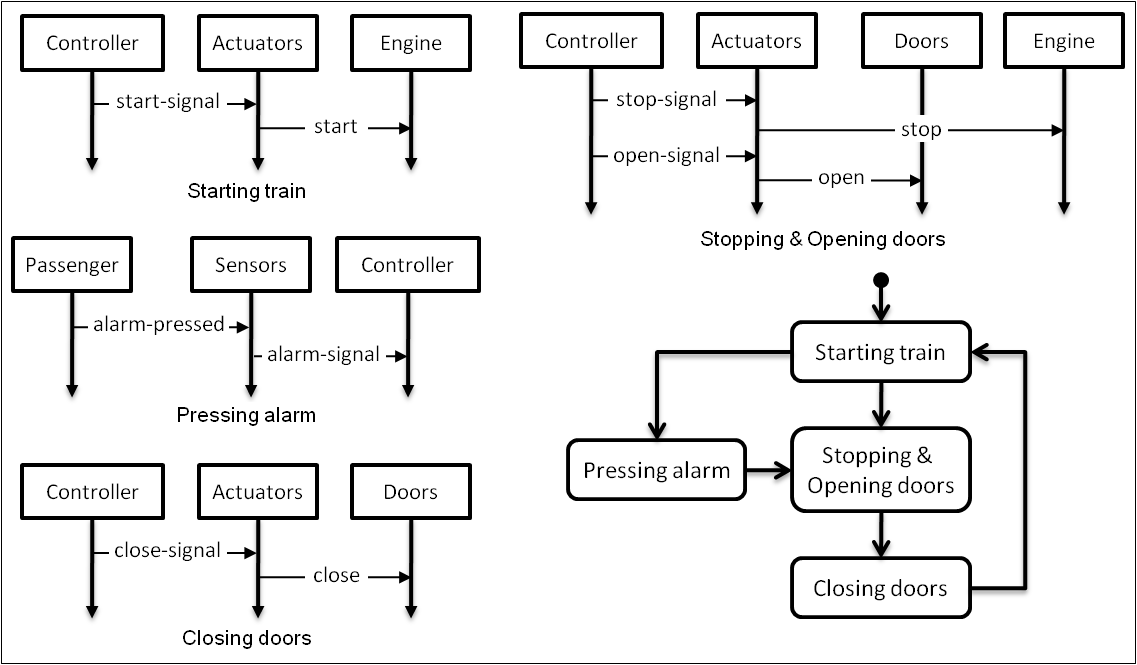
\includegraphics[trim=2mm 2mm 2mm 2mm, clip]{src/2-framework/images/train-hmsc}
}
\caption{A high-level Message Sequence Chart for the train system.\label{image:train-hmsc}}
\end{figure}

The two following sections define the trace semantics of hMSCs. We first restrict to hMSCs composed of bMSCs only before taking finer-grained hMSCs into account. 

\subsubsection*{hMSCs composed from bMSCs only\label{subsubsection:hMSC-bMSC-only}}

A trace semantics for hMSCs provides an answer to the question: \emph{what traces are captured by a hMSC?} This apparently simple question has a fairly complex answer. The reasons are manifold; we summarize here then slightly extend the characterization provided in~\cite{Uchitel:2004}.

\noindent \textbf{Bounding hMSCs} -- As explained in \cite{Henriksen:2000}, some hMSCs do not define regular languages. In that case, they have sets of traces that cannot be captured by a LTS. Our framework must therefore be restricted to regular hMSCs. Under a total ordering of events inside bMSCs, hMSCs are regular. Under a partial ordering, a sufficient condition for a hMSC to be regular is that it does not contain a cycle in which two disjoint sets of agents interact independently of each other. We will make the assumption of \emph{bounded} hMSCs in the sequel.

\noindent \textbf{Composing bMSCs} -- In addition to the partial or total ordering of events in bMSCs, two possibilities arise as to how a system evolves from a bMSC to another inside a hMSC. The first one, called \emph{strong sequential composition}, assumes that all agents wait until all events of a bMSC have occurred before moving to the next one. This means that there is an implicit synchronization scheme used by the agents to know when a scenario has been completed. The other one, called \emph{weak sequential composition}, allows an agent to move from a bMSC to another one without having to synchronize with the other agents. 

In view of the independence between the assumptions of partial/total event ordering and weak/strong sequential composition, four combinations actually exist. To keep things simple enough and avoid bizarre concurrency models\footnote{in particular, such models are very sensitive to the decomposition of a hMSC into bMSCs. For example splitting a bMSC node into smaller bMSCs might change the set of accepted traces of the hMSC.}, we do not consider partial (resp. total) ordering with strong (resp. weak) sequential composition. In the sequel, therefore, strong (resp. weak) sequential composition will entail total (resp. partial) ordering of MSC events. In the sequel, we will refer to this as the \emph{stable composition} hypothesis. 

\noindent \textbf{Trace semantics} -- Under the assumption of bounded hMSC with stable composition, the trace analysis for hMSCs is very similar to MSCs. It leads to language relations similar to the ones given for the latter in Section~\ref{subsection:background-positive-scenarios} -- see (\ref{equation:msc-composition-1}) and (\ref{equation:msc-composition}) in particular:
\begin{align}
\mathcal{L}_{strong}(H) & \subseteq \mathcal{L}_{weak}(H) \\
\mathcal{L}_{weak}(H) & \subseteq \mathcal{L}(H_{\downarrow Ag_1} \parallel \ldots \parallel H_{\downarrow Ag_n})
\label{equation:hsmc-traces-by-agent-composition}
\end{align}

The sets of traces $\mathcal{L}_{strong}(H)$ and $\mathcal{L}_{weak}(H)$ result from the scenarios that can be ``produced'' by the hMSC under strong and weak sequential composition, respectively. Such ``production'' simply results from the concatenation of bMSCs along paths admissible by the hMSC.

For example, concatenating the bMSCs \emph{Starting train}, \emph{Pressing alarm} and \emph{Stopping} \& \emph{Opening the doors} in the hMSC of Fig.~\ref{image:train-hmsc} leads to the MSC of Fig.~\ref{image:train-scenario-all-agents}. 

Such MSC $M$ defines the set of traces $\mathcal{L}_{total}(M)$ and $\mathcal{L}_{partial}(M)$, see Section~\ref{subsection:background-positive-scenarios}. The trace semantics of a hMSC $H$ is defined in terms of all possible MSCs that it produces: 
\begin{align*}
\mathcal{L}_{strong}(H) &= \bigcup_{M \in H} \mathcal{L}_{total}(M) \\
\mathcal{L}_{weak}(H) &= \bigcup_{M \in H} \mathcal{L}_{partial}(M)
\end{align*}
\noindent where $M \in H$ means ``the MSC $M$ can be produced by a path in $H$''. The language $\mathcal{L}_{weak}$ corresponds to the notion of \emph{trace model of a hMSC} in~\cite{Uchitel:2004}.

Another way of defining the set of traces of a hMSC consists in considering the local perspective of the agent timelines. This is similar to what has been done for MSCs in relation (\ref{equation:msc-composition}) and leads to the right term in~(\ref{equation:hsmc-traces-by-agent-composition}). There, hMSC traces are computed as the composition of local agent traces $H_{\downarrow Ag_i}$ (see below). The composition of such LTS for each agent corresponds to the notion of \emph{minimal architecture model} in~\cite{Uchitel:2004}. We denote it by $\mathcal{L}_{arch}(H)$:
\begin{align}
\mathcal{L}_{arch}(H) &= \mathcal{L}(H_{\downarrow Ag_1} \parallel \ldots \parallel H_{\downarrow Ag_n})
\end{align}

To sum up, defining the trace semantics of a hMSC $H$ leads to considering three sets of traces, namely $\mathcal{L}_{strong}(H)$, $\mathcal{L}_{weak}(H)$ and $\mathcal{L}_{arch}(H)$. The former two consider the global perspective of the hMSC whereas the latter consider the local perspective of agent timelines. Moreover, $\mathcal{L}_{strong}(H)$ assumes a strong sequential composition of bMSC nodes with total event ordering whereas $\mathcal{L}_{weak}(H)$ and $\mathcal{L}_{arch}(H)$ both assume weak sequential composition and partial ordering. These three languages are related as follows:
\begin{align*}
&\mathcal{L}_{strong}(H) \subseteq \mathcal{L}_{weak}(H) \subseteq \mathcal{L}_{arch}(H)
\end{align*}

In practice, compositional algorithms allow capturing these three languages with LTS:
\begin{itemize}
\item An algorithm for synthesizing a LTS for $\mathcal{L}_{arch}(H)$ may be found in \cite{Uchitel:2003}. For a given agent $Ag_{i}$, the LTS $H_{\downarrow Ag_i}$ is synthesized by connecting the LTSs $M_{\downarrow Ag_i}$ corresponding to each bMSC $M$ with $\tau$ transitions, according to their possible continuations given by hMSC edges. 

This construction is illustrated in Fig.~\ref{image:train-controller-synthesis} for the hMSC in Fig.~\ref{image:train-hmsc} and the \artifact{Controller} agent. The resulting LTS can be further simplified by removing $\tau$ transitions and minimizing the result.
\vspace{0.4cm}
\begin{figure}[H]\centering
\scalebox{0.85}{
  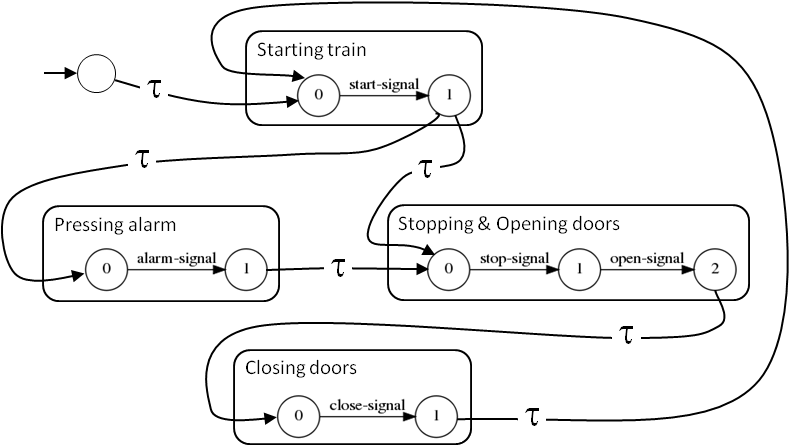
\includegraphics[trim=0mm 0mm 0mm 0mm, clip]{src/2-framework/images/train-controller-synthesis}
}
\caption{Synthesis of the \emph{Controller} LTS from the hMSC of Fig.~\ref{image:train-hmsc}.\label{image:train-controller-synthesis}}
\end{figure}

\item Thanks to the simplicity of the model with strong sequential composition, $\mathcal{L}_{strong}(H)$ can be captured in a similar way. The linear event trace defined by each MSC is used instead of $M_{\downarrow Ag_i}$ in the algorithm above.

\item The synthesis of a LTS for $\mathcal{L}_{weak}(H)$ is more complex because the sequencing and synchronization of bMSCs must be constrained to fit the semantics. A synthesis algorithm can be found in~\cite{Uchitel:2004}.
\end{itemize}

An important difference should be noted among the relations between MSC languages and those on hMSC languages. For similarity with hMSCs, let $\mathcal{L}_{arch}(M)$ denote an architecture model for MSCs:
\begin{align*}
\mathcal{L}_{arch}(M) = \mathcal{L}(M_{\downarrow Ag_1}\parallel\ldots\parallel M_{\downarrow Ag_n})
\end{align*}

\noindent For a MSC $M$ and a hMSC $H$ the language relations are, respectively:
\begin{align}
&\mathcal{L}_{total}(M) \subseteq \mathcal{L}_{partial}(M) = \mathcal{L}_{arch}(M) \label{relation:msc-total-language}\\
&\mathcal{L}_{strong}(H) \subseteq \mathcal{L}_{weak}(H) \subseteq \mathcal{L}_{arch}(H) \label{relation:hmsc-strong-language}
\end{align}

Note the equality between $\mathcal{L}_{partial}(M)$ and $\mathcal{L}_{arch}(M)$ in (\ref{relation:msc-total-language}) and the set inclusion between $\mathcal{L}_{weak}(H)$ and $\mathcal{L}_{arch}(H)$ in (\ref{relation:hmsc-strong-language}). 

The traces in $\mathcal{L}_{arch}(H) \setminus \mathcal{L}_{weak}(H)$ capture the set of \emph{implied} scenarios of a hMSC specification~\cite{Alur:2000, Uchitel:2004}. Implied scenarios occur when a system is designed globally while implemented component-wise. They capture traces that follow different paths in the hMSC when projected on individual agent timelines. Implied scenarios will be mostly ignored in the thesis; we will discuss their impact on our inductive technique in Section~\ref{section:inductive-correctness}.

\subsubsection*{hMSCs composed from finer-grained hMSCs\label{subsubsection:hMSC-with-sub-hMSC}}

A hMSC node may refer to a finer-grained hMSC instead of a bMSC. To take this into account in the trace semantics given previously, we must decide how a sub-hMSC is to be ``connected'' with its father. To keep a consistent framework in terms of synchronization hypotheses, we require such sub-hMSC to have, in addition to its initial state, a terminating state to which at least one node is connected. For simplicity, we forbid nodes with no outgoing transition. 

Under those assumptions, it is fairly easy to unfold a compound hMSC into another where all refined nodes are basic MSCs. The trace semantics remains unchanged and is defined in terms of the latter ``flat'' hMSC. 

In practice, this flat hMSC must not be explicitly constructed when the LTS for $\mathcal{L}_{arch}$ is synthesized. Under our assumptions, the LTSs capturing the traces of finer-grained hMSCs have only one initial state and only one terminating state. Therefore, they can connected with $\tau$ transitions in the same way as the LTSs $M_{\downarrow Ag_i}$ in the synthesis algorithm of previous section. A similar argument applies for $\mathcal{L}_{strong}$.

\subsection{Consistency between the scenario and state machine views\label{subsection:background-scenario-consistency}}

The trace semantics of scenarios can be explicitly related to the one of agent and system state machines. This section defines consistency rules between those two views, thereby explaining the similarity between relations (\ref{equation:system-composition}), (\ref{equation:msc-composition}) and (\ref{equation:hsmc-traces-by-agent-composition}).

\subsubsection*{Positive MSCs}

Consider a system composed of $n$ agents whose behavior is modeled by $\system$. Let $M$ denote a positive MSC illustrating interactions among them. $M$ and $S$ are said to be \emph{consistent} if the following conditions hold:

\noindent \textbf{Structural consistency} -- This condition requires $M$ and $S$ to agree on the set of agents and their respective interfaces. The MSC may actually illustrate interactions among a proper subset of system agents. However, labels along a timeline must be a subset of the alphabet of the corresponding agent.

\noindent \textbf{Consistent agent view} -- This condition states that the traces defined by a timeline in the MSC must be traces accepted in the LTS modeling the behavior of the corresponding agent. For each agent $Ag_i$, we must have:
\begin{align}\mathcal{L}(M_{\downarrow Ag_i}) & \subseteq \mathcal{L}(Ag_i)\label{condition:consistent-agent-view}.\end{align}

\noindent \textbf{Consistent system view} -- This third condition states that all linearizations of the MSC must be accepted traces in the LTS modeling the behavior of the composed system:
\begin{align}\mathcal{L}(M) & \subseteq \mathcal{L}(S)\label{condition:consistent-system-view},\end{align}
where $\mathcal{L}(M) = \mathcal{L}(M_{\downarrow Ag_1} \parallel \ldots \parallel M_{\downarrow Ag_n})$

\subsubsection*{Negative MSCs}

A negative MSC $N = (P,e)$ and a system $\system$ are said to be consistent if the following conditions hold:

\begin{itemize}
\item $N$ and $S$ are \emph{structurally} consistent, in a similar sense to what has been said for positive MSCs,

\item the precondition $P$ and $S$ are consistent; this requires conditions (\ref{condition:consistent-agent-view}) and (\ref{condition:consistent-system-view}) to hold for $P$,

\item the system may not exhibit any trace captured by the negative MSC, that is,
\begin{align}\mathcal{L}^{-}(N) \cap \mathcal{L}(S) &= \emptyset~,\label{condition:consistent-system-view-neg}\end{align}
which provides the negative counterpart of (\ref{condition:consistent-system-view}).
\end{itemize}

\subsubsection*{Scenario collections}

A scenario collection $Sc = (S^+,S^-)$ and a system $S$ are said to be consistent if and only if each positive and each negative MSC of the collection is itself consistent with $S$. 

Conditions (\ref{condition:consistent-system-view}) and (\ref{condition:consistent-system-view-neg}) can be formulated in terms of the positive and negative languages of the collection as follows:
\begin{align}
&\mathcal{L}^+(Sc) \subseteq \mathcal{L}(S) \\
&\mathcal{L}^-(Sc) \cap \mathcal{L}(S) = \emptyset
\end{align}

Observe that a scenario collection may only be consistent if all its scenarios, positive or negative, start in the same system state.

A set $S^+$ of positive scenarios and a set $S^-$ of negative scenarios are consistent with each other if there exists a system which is consistent with them taken as a collection $Sc = (S^+,S^-)$. 

A necessary condition for a scenario collection $Sc = (S^+,S^-)$ to be consistent is the disjointness of positive and negative traces:
\begin{equation}
\mathcal{L}^+(Sc) \cap \mathcal{L}^-(Sc) = \emptyset
\end{equation}

This condition is not sufficient, however, as structural consistency is not guaranteed.

\subsubsection*{High-level MSCs}

A hMSC $H$ and a system $\system$ are said to be consistent if the following conditions hold:
\begin{itemize}
\item $H$ and $S$ are \emph{structurally} consistent,
\item $\mathcal{L}(H_{\downarrow Ag_i}) \subseteq \mathcal{L}(Ag_i)$ for each agent $Ag_i$,
\item $\mathcal{L}_{arch}(H) \subseteq \mathcal{L}(S)$,
\end{itemize}
where $\mathcal{L}_{arch}(H) = \mathcal{L}(H_{\downarrow Ag_1} \parallel \ldots \parallel H_{\downarrow Ag_n})$

These conditions are the counterpart of those given previously for MSCs. They have a similar interpretation, \emph{mutatis mutandis}. 

Last, it is sometimes convenient to distinguish between a hMSC that describes all behaviors of a system and one that only illustrates a subset of them. This leads to the notion of hMSC completeness. 

A hMSC $H$ is \emph{complete} for a system $\system$ if it is consistent with it and defines the same language, that is, if the following condition holds:
\begin{align}
\mathcal{L}_{arch}(H) &= \mathcal{L}(S)
\end{align}


\section{State-based assertions on fluents\label{section:background-fluents}}

Miller and Shanahan define fluents as ``\emph{time-varying properties of the world that are true at particular time-points if they have been initiated by an event occurrence at some earlier time-point, and not terminated by another event occurrence in the meantime. Similarly, a fluent is false at a particular time-point if it has been previously terminated and not initiated in the meantime}''~\cite{Miller:2002}.

Fluents will allow us to integrate event-based and state-based specification styles within a simple framework~\cite{Giannakopoulou:2003}. 

A fluent $Fl$ is thus a proposition defined by a set $Init_{Fl}$ of initiating events, a set $Term_{Fl}$ of terminating events, and an initial value $Initially_{Fl}$ that can be true or false. The sets of initiating and terminating events must be disjoint. The concrete syntax for fluent definitions is the following~\cite{Giannakopoulou:2003}:

\begin{center}
fluent $Fl = \textless Init_{Fl}, Term_{Fl} \textgreater $ initially $Initially_{Fl}$
\end{center}

In our train example, the safety goal ``\emph{\texttt{Doors shall remain closed while the train is moving}}'' suggests two fluents defined as follows:

\begin{center}
fluent $Moving = \textless \{start\}, \{stop\} \textgreater $ initially \emph{false} \\
fluent $DoorsClosed = \textless \{close\}, \{open\} \textgreater $ initially \emph{true} \\
\end{center}

\subsection{Fluent values along single traces\label{subsection:background-fluents-single-traces}}

In terms of our trace semantics, a fluent $Fl$ will be \emph{true} after a finite trace $s$ if and only if one of the following conditions hold~\cite{Giannakopoulou:2003}:

\begin{enumerate}
\item $Fl$ holds initially and no terminating event has occurred in $s$.
\item Some initiating event has occurred in $s$ with no terminating event occurring since then.
\end{enumerate}

As sets of initiating and terminating events are disjoint, the value of a fluent after a given trace is deterministic. 

For example, the fluent \emph{Moving} is \emph{true} after the trace \artifact{<start stop start>}, but not after the empty trace $\lambda$ nor after \artifact{<start stop>}. 

As prefixes of traces are also traces, we may also think in terms of fluent values \emph{along} traces. This is illustrated in Fig.~\ref{image:fluent-values-along-a-trace} where the values of the two fluents introduced above are shown in the states of a LTS capturing a typical event trace for the train system. 

\begin{figure}[H]\centering
\scalebox{0.45}{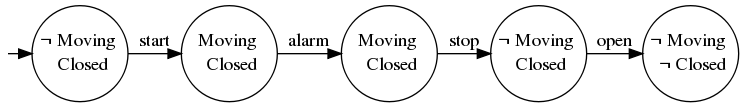
\includegraphics{src/2-framework/images/decorating-trace}}
\caption{LTS annotated with fluent values along a single trace (\artifact{Closed} is an abbreviate for \artifact{DoorsClosed}).\label{image:fluent-values-along-a-trace}}
\end{figure}

As the example suggests, for a set of fluents $\Phi$, an event trace yields an interpretation over $2^\Phi$, that is, an assignment of a Boolean value to each fluent in $\Phi$. We will call it \emph{fluent value assignment} throughout the thesis. 

For example, the maximal trace Fig. \ref{image:fluent-values-along-a-trace} yields the following fluent value assignment:
\begin{center}
\{\emph{Moving} $=$ \emph{false}, \emph{DoorsClosed} $=$ \emph{false}\}
\end{center}

\subsection{Fluent values along multiple traces}

We can similarly annotate the states of any LTS. The generalization consists in considering that a LTS state may be reached by a set of traces instead of a single one. Annotations therefore become \emph{sets} of fluent assignments, that is elements of the powerset $\mathcal{P}(2^\Phi)$ over $2^\Phi$. 

In particular, a state might be reached by a trace yielding a fluent \emph{true}, while another trace reaching it would yield the same fluent \emph{false}. Note that even in presence of a possibly infinite number of traces, the set of all possible annotations is itself finite. $\mathcal{P}(2^\Phi)$ actually coincides with the set of propositional formulas over fluents. It appears convenient to consider state annotations as such formulas, where \emph{false} then corresponds to an empty set of fluent assignments (i.e. an unreachable state) and \emph{true} corresponds to the set of all possible assignments. Such state annotations will be called \emph{state invariants}; they encode assertions that always hold when the LTS state is visited. Fig.~\ref{image:fluent-values-along-multiple-traces} shows an example of LTS annotation with state invariants.

\begin{figure}[H]\centering
\scalebox{0.45}{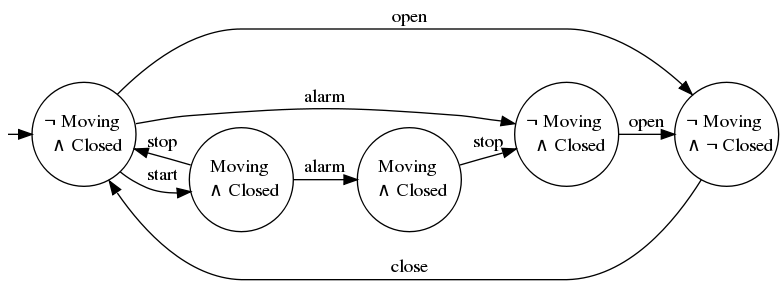
\includegraphics{src/2-framework/images/decorating-lts}}
\caption{Fluent values along multiple traces (\artifact{Closed} is an abbreviate for \artifact{DoorsClosed}).\label{image:fluent-values-along-multiple-traces}}
\end{figure}

A fixpoint algorithm for decorating LTS with fluent value assignments appeared in~\cite{Damas:2005}. This algorithm was generalized for generating weakest state invariants in \cite{Damas:2009, Damas:2011}. Very roughly, it consists in annotating the LTS initial state with an initial invariant according to fluent initial values; invariants are then propagated along LTS transitions, according to fluent definitions, and accumulated in states through Boolean disjunction, until a fixpoint is reached. 

Binary decision diagrams~\cite{Bryant:1986} can be used for concisely encoding and efficiently manipulating Boolean formulas (see Chapter~\ref{chapter:tool-support}). This algorithm has been further generalized in~\cite{Damas:2011} for handling other kinds of decorations than state invariants.

\subsection{Integrating fluents in multi-view models}

Fluents provide a general mechanism for integrating event-based and state-based specifications. We may thus them for integrating agents, their state machines, and scenarios. The next section extends such integration by introducing fluent-based goals and domain properties.

We will restrict our use of fluents to the ones that are monitorable and controllable by the agents forming the system~\cite{Letier:2002}. 

A fluent is \emph{monitorable} by an agent if all its initiating and terminating events can be either sent or received by this agent. It is \emph{controllable} if all initiating and terminating events can be sent by the agent. 

Our restriction to fluents that are monitorable or controllable by system agents is motivated by the need for specifications  to be realizable by the agents involved in them~\cite{Letier:2002}.

\section{Declarative goals and domain properties\label{section:background-goals}}

A \emph{goal} is a prescriptive statement of intent whose satisfaction requires the collaboration of agents forming the system. Unlike goals, \emph{domain properties} are descriptive statement about the environment -- such as physical laws, organizational rules, etc. Goals are structured in AND/OR refinement graphs that show how they contribute to each other~\cite{VanLamsweerde:2000}.

Section~\ref{subsection:background-goals-as-fltl-assertions} formalizes goals and domain properties in fluent linear temporal logic (FLTL). Their integration with state machines and scenarios is discussed in Section~\ref{subsection:background-goals-consistency}. Section~\ref{subsection:background-property-and-tester-automata} then presents how all system traces satisfying (resp. violating) a safety goal can be specified through a property (resp. a tester) automata.

\subsection{Properties as FLTL assertions\label{subsection:background-goals-as-fltl-assertions}}

Goals and domain properties can be formalized in Linear Temporal Logic (LTL). Admissible system histories are thereby specified in a declarative and implicit way~\cite{VanLamsweerde:2009}. We will focus on propositional LTL here. In addition to the usual propositional constructs, LTL provides connectives for temporal referencing~\cite{Manna:1992}: 

\begin{itemize}
\item $\circ$ (at the next smallest time unit), 
\item $\diamond$ (some time in the future), 
\item $\square$ (always in the future), 
\item $\rightarrow$ (implies in the current state), 
\item $\Rightarrow$ (always implies), 
\item $\mathcal{U}$ (always in the future until), 
\item $\mathcal{W}$ (always in the future unless)
\end{itemize}

A system history is commonly seen in LTL as a temporal sequence of system states. Atomic LTL propositions then refer to state formulas (as, e.g. in the SPIN model-checker~\cite{Holzmann:1997}). In our event-based setting, a system history will be seen as a trace, that is, a temporal sequence of events. 

To integrate the state-based and event-based paradigms, we will use a flavor of LTL known as Fluent Linear Temporal Logic (FLTL), where atomic propositions are fluents~\cite{Giannakopoulou:2003}. FLTL proves convenient for specifying state-based temporal logic properties over the event-based operational model given by scenarios and state machines. 

For example, the safety goal ``\emph{Doors shall remain closed while the train is moving}'' of our running example can be formalized in terms of the $Moving$ and $DoorsClosed$ fluents, defined in the previous section:
\begin{center}
\artifact{Maintain[DoorsClosed While Moving]} = $\square(Moving \rightarrow DoorsClosed)$
\end{center}

Properties formalized in temporal logic are commonly classified as \emph{liveness} or \emph{safety} properties~\cite{Alpern:1986}. Liveness refers to ``\emph{something good will eventually happen}'' whereas safety refers to  ``\emph{something bad may never happen}''. The thesis will focus on safety properties for the following reasons:
\begin{itemize}
\item Reasoning about liveness requires considering the acceptance of infinite execution traces; this is outside the expressiveness of our LTS characterization and regular languages in general. In contrast, if ``something bad'' happens it must do so after a finite sequence of events, and is irremediable~\cite{Alpern:1986, Giannakopoulou:1999}.
\item The thesis focusses on requirements engineering models. To be realizable by agents, the properties assigned to them must be bounded as \emph{maintain} or \emph{bounded achieve} specifications \cite{Letier:2002}; these correspond to safety properties.  
\end{itemize}

\subsection{Consistency between the behavioral and intentional views\label{subsection:background-goals-consistency}}

Consider a safety property $G$ and a system $\system$. Let $\mathcal{L}^{-}(G)$ denote the set of event traces violating the property and $\mathcal{L}^{+}(G)$ those not violating it. We discuss how these languages can be captured with automata in the following section.

The system $S$ and the property $G$ are consistent if and only if the following condition holds:
\begin{equation}
\mathcal{L}(Ag_1 \parallel \ldots \parallel Ag_n) \cap \mathcal{L}^{-}(G) = \emptyset
\label{equation:state-machines-and-goals-consistency}
\end{equation}

The above relation requires the system to exclude any trace violating the property. This relation is the one commonly used in model checking, provided that $\mathcal{L}^{-}(G)$ actually amounts to $\mathcal{L}^{+}(\neg G)$ \cite{Clarke:1989}. In other words, $\mathcal{L}^{-}(G)$ actually captures the set of traces satisfying the negation of the safety property.

We also consider consistency rules between goals and scenarios, as follows:
\begin{itemize}
\item Behaviors illustrated in positive scenarios may not violate safety goals. A more formal expression of this depends on the concrete form of scenario specification (scenario collection or hMSC) and on hypotheses about event ordering and weak or strong bMSC synchronization. It is similar to relation (\ref{equation:state-machines-and-goals-consistency}), \emph{mutatis mutandis}.
\item A negative scenario $N$ \emph{illustrates} the violation of a safety goal, say $G$, if the following condition holds:
\begin{equation}
\mathcal{L}^{-}(N) \subseteq \mathcal{L}^{-}(G)
\end{equation}
\noindent that is, if the negative traces it defines are among those prescribed by the safety goal.
\end{itemize}

\subsection{Property and tester automata\label{subsection:background-property-and-tester-automata}}

For a safety property $G$, the sets of traces $\mathcal{L}^{+}(G)$ and $\mathcal{L}^{-}(G)$ can be specified through automata. The former correspond to the notion of \emph{property} automaton in \cite{Letier:2005, Letier:2008} while the latter corresponds to the one of \emph{tester} automaton in \cite{Giannakopoulou:2003}. We consider the construction of each of them in turn.

The negative language $\mathcal{L}^{-}(G)$ cannot be captured with a pure LTS as it is not prefix-closed. For example, the trace \artifact{<start open>} violates the safety goal for the train system; it thus belongs to $\mathcal{L}^{-}(Maintain[\mbox{\emph{DoorsClosed While Moving}}])$. However, \artifact{<start>} does not violate it (yet). 

On the other hand, a safety property can only be violated after a finite trace, and remains violated after that; $\mathcal{L}^{-}(G)$ is thus suffix-closed. 

Let us consider the positive language $\mathcal{L}^{+}(G)$, that is, the set of all possible system traces that do \emph{not} violate the property. This language includes at least all traces that, up to one event, do not violate the property; it also includes all their prefixes, but not all their suffixes. Thus, $\mathcal{L}^{+}(G)$ is prefix-closed, and can be specified through a LTS. 

$\mathcal{L}^{-}(G)$ and $\mathcal{L}^{+}(G)$ turn to be \emph{complement} of each other, that is, 

\begin{equation}
\mathcal{L}^{+}(G) = \Sigma^{*} \setminus \mathcal{L}^{-}(G)
\end{equation}

The complement of a regular language is known to be a regular language as well~\cite{Hopcroft:1979}. Hence, both can be modeled through standard automata. 

In contrast, the complement of a prefix-closed language is not prefix-closed, as illustrated in our example. Moreover, the complement of a language is easily obtained by flipping accepting and non-accepting states of its automaton, provided the latter has a complete transition function. 

Fig.~\ref{image:tester-and-property-automata} shows two complement automata, where accepting states are represented by double circles.

\begin{figure}[H]\centering
\scalebox{0.40}{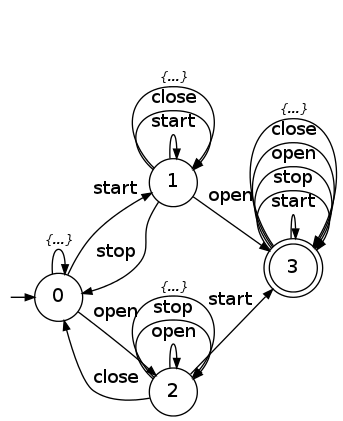
\includegraphics{src/2-framework/images/tester-automaton}}
\scalebox{0.40}{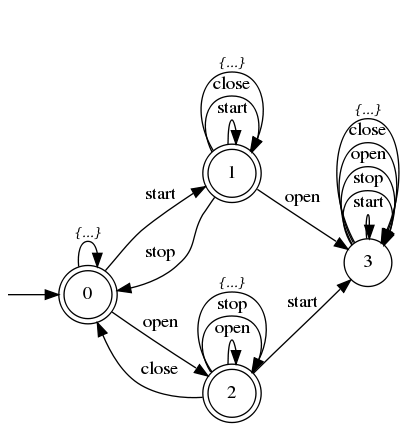
\includegraphics{src/2-framework/images/property-automaton}}
\caption{Tester ($\mathcal{L}^{-}$ at left) and property ($\mathcal{L}^{+}$ at right) automata for \artifact{Maintain[DoorsClosed While Moving]}, as complements of each other.\label{image:tester-and-property-automata}}
\end{figure}

A procedure for computing tester automata in the case of safety properties is given in \cite{Giannakopoulou:2003}. Very roughly, it consists in composing a B\"uchi automaton that captures the negation of the state-based FLTL property with fluent automata capturing the event-based semantics of fluents, plus a synchronizer between both. 

Given a pure safety property, a canonical form for this automaton can been found; the latter is deterministic, has a complete transition function, and a unique sink accepting state reached by all traces violating the property~\cite{Giannakopoulou:2003}. An example of such tester automaton for the safety goal of the train system is given on the left of Fig.~\ref{image:tester-and-property-automata}. One can check that all traces leading to the accepting state capture situations where the train is moving with doors open. 

The \emph{property} automaton can thus be obtained by flipping accepting and non-accepting states of the tester (as shown on the right of the same figure). 

A few remarks are in order here:
\begin{itemize}
\item In the LTSA tool \cite{Magee:1999} and related literature, a tester LTS with an error state is used instead of the tester automaton presented here. Similarly, \cite{Letier:2005, Letier:2008} actually use a property LTS that corresponds to the tester LTS from which the error state has been removed, instead of the property automaton shown here. Our automata variants are better suited here in view of the formalization of inter-model consistency rules expressed in terms of set-theoretic operators on languages. 

\item The tester and property automata, together with the procedure for computing them, are always defined ``up to a given alphabet'' or ``under the assumption of a given agent or system''. This is the intended meaning of the transitions labeled ``\emph{\{...\}}" in Fig.~\ref{image:tester-and-property-automata}. The reason is that some temporal properties, in particular those referring to the FLTL \emph{next} operator, are not closed under stuttering~\cite{Lamport:1994}. This means that their satisfaction may be affected by the insertion or removal of unobservable events. Which events are relevant may depend on additional hypotheses about how goals relate to agent behaviors -- e.g, whether they are under the responsibility of a single agent or are properties to be met by the global system. Fixing those ``relevant events'' by filling the ``\emph{\{...\}}" placeholder is required for meeting the temporal logic semantics when composing tester and property automata. 

For simplicity in the thesis, we will consider that safety properties must be met by the global system. Therefore, the relevant events are the alphabet of the whole system, say $\Sigma$. A placeholder then must be replaced by a transition for each event in $\Sigma$ except those already labeling an outgoing transition from the same state.
\end{itemize}

\section{Process models as guarded high-level message sequence charts\label{section:background-process-models}}

Process models capture tasks performed by agents together with their control flow. The aim here is to model work processes for effective software support \cite{Dumas:2005}. A process lifecycle typically includes \emph{process modeling} \cite{OMG:2004, OMG:2008, Clarke:2008, Damas:2009}; \emph{process enactment} \cite{Manolescu:2002, Buhler:2005, Sauer:2006}; \emph{process monitoring} \cite{Muehlen:2000}; and \emph{process restructuring} based on monitored data. 

Process models considered in the thesis will be formalized as guarded high-level message sequence charts (g-hMSC), an extension of hMSCs with guards on fluents \cite{Damas:2009}. Guarded hMSCs capture \emph{decision-based processes} where decisions relying on the state of the process environment regulate the nature of the subsequent tasks and their composition. 

An example of g-hMSC is given in Fig.~\ref{image:scheduler-ghmsc} for the meeting scheduling case study. Such processes are frequently found in medical therapies, for example.  

\begin{description}
\item[A task] is a unit of work to be performed by collaboration of agents involved in the process. 

Task nodes in a g-hMSC may be refined either by a MSC or by a finer-grained g-hMSC. For example, the \texttt{InitiateMeeting} task in Fig.~\ref{image:scheduler-ghmsc} is refined into a MSC illustrating interactions between the initiator, the scheduler and participants. 

A g-hMSC defines a strong sequential composition of task nodes; a total ordering of all events also applies inside MSCs (see Section \ref{subsection:background-hmsc}). This assumes an implicit synchronization scheme used by the agents to know when tasks are starting and terminating. Automated process enactment typically provides such support through agent worklists, reminders sent to them, and the like. 

Such synchronization is kept implicit in the process model. However, for reasoning about timing of tasks and manipulating the traces that a g-hMSC accepts (see Chapter \ref{chapter:deductive}), it proves convenient to associate with a task special events for denoting its start and end. For a task $T$ such events will be denoted by $T_{start}$ and $T_{end}$, respectively. They correspond to \emph{broadcasting} interactions, which implies that all agents are supposed to monitor them.

\item[A decision node] states specific conditions for the tasks along outgoing branches to be performed. Each outgoing branch is labeled by a Boolean expression on fluents, called \emph{guard}. A guard must be evaluated to true for the corresponding branch to be followed.

For example, the guards in Fig.~\ref{image:scheduler-ghmsc} refer to the three fluents: \emph{second\_cycle}, \emph{date\_conflict} and \emph{resolve\_by\_weakening}. The former is defined as below; the two others are to be defined in terms of events introduced in refinements of other tasks.
\begin{center}
fluent $second\_cycle = \textless \{ ExtendDateRange_{end}, \newline WeakenConstraints_{end} \},
 \{ InitiateMeeting_{end} \} \textgreater $\\
\end{center}

Instead of initial values for fluents, a g-hMSC is given an \emph{initial condition} that constrains the acceptable initial fluent values. This allows processes to be modelled where different instances can start in different states; initial values for fluents can then be defined at instance level rather than at class level. The initial condition will be denoted by $C_0$. In our example, it might be defined as follows:
\begin{align*}
C_0 = \neg second\_cycle \wedge \neg date\_conflict \wedge \neg resolve\_by\_weakening
\end{align*}

\end{description} 

The trace semantics of guarded hMSCs will be defined in Chapter \ref{chapter:deductive} together with synthesis techniques to derive them as state machines for automated reasoning.

\section{Model synthesis opportunities\label{section:background-discussion}}

We close this chapter with an overview of existing model synthesis techniques and opportunities offered by the framework defined here. Model synthesis outside the boundaries of the present framework is discussed in chapter~\ref{chapter:discussion}.

As stated earlier, the term ``model synthesis'' can be interpreted differently according to the objectives behind its use. In particular, we have already made a distinction between analysis-driven synthesis and multi-view model synthesis. In the first, synthesized models are for the \emph{machine}, and are typically used by a model-checker, an animator, a code generator, and so on. If not hidden to the end-user, their primary intent is not to be manipulated by her. In the second, models are for \emph{humans} and are used for thinking about, designing or documenting a system. Synthesized models aim at completing a multi-view system description, at semi-automatically validating it with the user, or both. Here, therefore, models are intended to be shown to users and understood by them.

We have said that the distinction between both is fuzzy. The reason is that analysis-driven synthesis proves useful for supporting a user-oriented completion and/or validation of multi-view system descriptions. A model-checker, for example, can be used to check the consistency between a safety goal and, say, a hMSC. However, the counter-example it generates can effectively been used to enrich the scenario description with a negative scenario illustrating the violation of the goal. Looking at model-checker internals shows analysis-driven synthesis techniques (e.g., from hMSC to LTS), while looking at its use -- maybe hidden use -- for helping building complete and consistent models shows multi-view synthesis techniques. We shortly describe additional examples of both kinds below.

TODO: add a note about the fact that analysis-driven synthesis is (seems?) necessarily deductive, while some kind of induction is often used in multi-view synthesis.

\subsection*{Analysis-driven synthesis}

The technique from \cite{Uchitel:2003}, presented in section~\ref{subsection:background-hmsc}, can be interpreted as synthesizing agent state machines from a hMSC. However, the technique is entirely deductive; it generates a minimal LTS for each agent, that is, a state machine that precisely captures the agent traces defined in the hMSC. Of course, inter-model consistency rules between the hMSC and generated state machines are respected by construction.  The authors' motivation is to be able to model-check or animate a hMSC specification. In that sense, state machines are not intended to be seen or manipulated directly by the end-user.

In chapter~\ref{chapter:deductive} of the present thesis, we extend our framework with guarded process models. The latter take the form of hMSCs to which decision nodes are added and we provide a declarative trace-based semantics for such models. The chapter also describes a synthesis algorithm for computing accepted traces as a LTS. This algorithm enables reusing a trace-based model-checker ala LTSA~\cite{Magee:1999} for guarded models.

\subsection*{Multi-view model synthesis}

In \cite{Uchitel:2004}, Uchitel explains how implied scenarios can be used to validate a hMSC specification, say $H$, with experts. Implied scenarios are all traces in $\mathcal{L}_{arch}(H) \setminus \mathcal{L}_{weak}(H)$, that is, scenarios that are not explicitly described in the hMSC, but that will necessarily be accepted in any system consistent with it. These scenarios are enumerated and submitted for classification as positive or negative by an expert. This allows to semi-automatically check the consistency between the system description given by the hMSC and the system composed of the agent state machines generated by the technique aforementioned \cite{Uchitel:2003}. As a notable side effect, classified scenarios enrich the initial scenario description. However, by definition, an implied scenario classified as negative hurts inter-model consistency, as it should be rejected by the system but could not be. In general, negative implied scenarios are a sign that agents and their interfaces should be refactored. 

A technique for synthesizing goals from a scenario collection is presented in~\cite{Damas:2006}. It consist in decorating MSC timelines with invariants on fluents monitored and controlled by the associated agent. From these invariants, goals are induced that respect two kinds of specification patterns, namely \emph{maintain goals} $\square(P \rightarrow Q)$ and \emph{immediate achieve goals} $\square(P \rightarrow \circ Q)$. Here also, inferred goals are submitted for classification by an expert. Accepted goals enrich the goal model while rejected ones call for enriching the scenario collection with a counter example. Thus, the technique helps enriching a multi-view system description while guaranteeing consistency. As it mostly relies on the availability of fluent invariants, the technique could be extended to infer goals from any annotated LTS, and hence, from agent state machines or a hMSC. 

In chapter~\ref{chapter:inductive-synthesis} of the present thesis, we describe an inductive technique for synthesizing agent state machines from scenario collections and hMSCs. Unlike \cite{Uchitel:2003} inferred models cover more behaviors than the hMSC. Also, information offered by the other models (fluents, goals, etc.) is used to guarantee inter-model consistency. The generalization process is guided by the end-user who is requested to classify additional scenarios as positive or negative system behaviors.  

